\documentclass[a4paper,10pt]{article}
\usepackage[english]{babel}
\usepackage[utf8]{inputenc}
%\usepackage[T1]{fontenc}
\usepackage[pdftex]{graphicx}
\usepackage{a4wide}
\usepackage[dvips,pdftex]{hyperref}

\usepackage{multicol}
\makeatletter
\newenvironment{tablehere}
{\def\@captype{table}}
{}

\newenvironment{figurehere}
{\def\@captype{figure}}
{}
\makeatother
\date{26/05/2008}
\begin{document}
	\begin{titlepage}
 		\title{Dynamical Handling of Straddle Carriers Activities on a Container Terminal in Uncertain Environment \\ \textit{- A Swarm Intelligence approach -}}
		
		\author{Stefan~Balev, Fr\'{e}d\'{e}ric~Guinand, Ga\"{e}tan~Lesauvage, Damien~Olivier}
			
	\end{titlepage}
	\maketitle
	
	\begin{abstract}

	 The CALAS project consists in a laser measure system allowing to localize precisely straddle carriers location in a box terminal. The information given by such a tool makes an optimization possible. In fact, a box terminal is an open system subject to dynamism, so many events can occur. They concern containers arrivals and departures. Within the terminal, straddle carriers are trucks which are able to carry one container at a time in order to move it through the terminal. We aim to optimize the straddle carriers handling to improve the terminal management. Moreover, missions come into the system in an impredictible way and straddle carriers are handled by human. They can choose to follow the schedule or not. For these reasons, the exact state of the system, i.e the exact location of boxes is unknown. The optimizing system that we try to build must be fail-safe and adaptative. So, in this context, how to devote a mission to a straddle carrier ? We propose a simulation approach using a meta-heuristic based on Ant Colony to resolve the scheduling problem.
	\\
	\end{abstract}
	

	
	\begin{figure*}[h]
	 
	\textbf{Keywords : } swarm intelligence, colored ant colony system, dynamic graph, multiple criteria optimization
	
	\end{figure*}


\begin{multicols}{2}
	
	\section*{System description}
		The CALAS project aims at localizing precisely handling truck on a box terminal. It uses a laser measure system and a software which allows to deal with the data sent by lasers. This project is the result of a collaboration between \textit{Laser Data Technology Terminal} company and the \textit{Terminaux de Normandie} company. The goal of the CALAS project is to know the state of the terminal in real time, meaning both containers and trucks location.
	
		A box terminal is divided into three main areas. Each part is a set of boxes rows where containers can be stacked up and these areas are linked by oriented roads. The first area is beside a channel where ships can tie to the dockside. It is an area bound to prepare the ship load or unload. The second area is used to load or unload trucks. The third part is a storing area linking the two others. Containers are moved into this area when a ship or a truck is unloaded, and containers are moved from this area when a ship or a truck is loaded. So, there are three kinds of missions:
		\begin{itemize}                                                                                                                    	\item Prepare a ship loading / unloading
			\item Prepare a truck loading / unloading
			\item Optimize storing area
		\end{itemize}
		
		The box terminal is an open system subject to dynamism. In fact, though a set of missions is known before starting the schedule, the main parts come into the system when the schedule has already been established. Moreover, trucks arriving time is not precisely known enough to forecast container delivery. If the truck is late, straddle carriers must wait for it to complete the mission, meanwhile, it can not accomplish another mission. Human behavior also affects the system because straddle carriers are handled by human drivers who can choose to follow the schedule or not.

	\section*{Vehicle Routing Problems classes}
 		The problem to solve belongs to many well known problem classes(see \cite{Larsen00}).

		The Vehicle Routing Problem with Time Windows (see \cite{Bianchi00}) (VRPTW) consists in visiting a set of cities by a set of capacitated vehicles, optimizing path length. For instance, an Italian factory produces toys. It has to deliver a set of stores in order to make the goods sold. These stores are spread all over the country and goods are carried by trucks. Trucks capacity is restricted and they all start from the factory depot. Deliveries can only be done during a defined time interval. If a truck comes too early, it will have to wait. A solution to this problem should minimize the global length of the trucks runs.
		
		The Dynamic VRPTW (DVRPTW) includes dynamism of the new orders. For the Italian factory example, if the stores can ask for deliveries when an already scheduled plan is running, then this problem belongs to DVRPTW class.

		These problems class concerns runs starting from the depot. Dynamic Pickup and Delivery Problem (see \cite{Mitrovic01,Mitrovic04,Mitrovic98}) (DPDP) consist in optimizing vehicles routes in order to pickup a load somewhere and deliver it to its destination. For instance, the mail delivery problem belongs to DPDP. A mail company employs a set of postmen. They have to pickup mails from the mail boxes of the company and deliver them to their recipients as soon as possible.

		Our problem belongs to the Dynamic Pickup and Delivery Problem with Time Windows. Straddle carriers can start from anywhere, ie. they don't have to start from the depot. Two problems must be solved:
		\begin{itemize}
 			\item Minimize straddle carriers moves : shortest path probem
			\item Minimize customers delays : scheduling problem
		\end{itemize} 
		In order to realize a good scheduling, the system must integrate the shortest path concept. In the same way, scheduling shortest paths trend to reduce straddle carriers moves.

	\section*{Ant Colony and Straddle Carrier Handling}
		Ant Colony (see \cite{Dorigo91,Dorigo97}) is a meta-heuristic which makes a solution appear thanks to the run of artificial ants into the solution space. The system is self-regulated. In fact, ants spread pheromone according to the solution quality (positive feedback) but the pheromone tracks evaporate progressively (negative feedback). The positive feedback makes the algorithm converge to a quality solution, and the negative feedback prevent it to block into a local extremum.

		Ant Colony with one colony provides a sorted list of missions to accomplish (see \cite{Montemanni04,Bullnheimer97,Bullnheimer99}). The problem is to set a mission to a specific straddle carrier.
		I have proposed to employ a solution using colored ants (see \cite{Bertelle02}). Every straddle carrier represent a colony with its own color. Ants are attracted by the pheromone of their own colony and repulsed by the pheromons of foreign colonies. These mecanisms will provide a sorted list of missions per every straddle carrier.
	
		The problem can be conceptualized as such: 
		\begin{itemize}
	 		\item let $M$ the set of missions to schedule. Every mission has a defined time window. We say that mission $m_i$ is prior to mission $m_j$ if the time window of $m_i$ starts before the one of $m_j$
			\item let $G$ $(V,A)$ an oriented graph where $V$ is the set of vertices and $A$ the set of arcs.
			\item $\forall \; m \in M$, $\exists$ $v \in V$
			\item $\exists$ $a(v_i , v_j) \in A$, if $m_i$ is prior to $m_j$
			\item $\forall \; c_i \in C$, where $C$ is the set of straddle carriers, $\exists \; vk_i \in V$. $\forall \; v \in V$, $\exists \; a(vk_i,v) \in A$.
			\item $\forall \; v \; \exists \;$ $e(h_i , v_j) \in E$, if $m_i$ is prior to $m_j$	
		\end{itemize}
		\begin{figurehere}
			\begin{center}
 				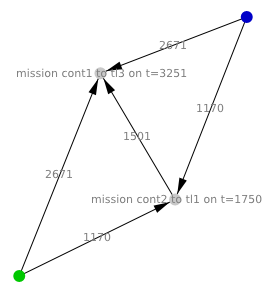
\includegraphics[width=80px]{Shemas/missiongraph.png} \\
				\caption{Mission graph for 2 straddle carriers and 2 missions }
				\label{missiongraph}
			\end{center}
		\end{figurehere}
		In this way, a graph is set and ants colony system is run to make the solution appear (see Fig. \ref{missiongraph}). The main algorithm is described on Fig. \ref{algo}. \\
		
		\begin{figurehere}
		 	\begin{flushleft}
			begin\\
			$\vert \;\;$for each colony c do\\
			$\vert \;\;\vert \;\;$for each ant of colony c do\\
			$\vert \;\;\vert \;\;\vert \;\;$to choose an unvisited destination according to the pheromone track\\
			$\vert \;\;\vert \;\;\vert \;\;$to move towards it according to the ant speed\\
			$\vert \;\;\vert \;\;\vert \;\;$to spread pheromone according to the destination quality\\
			$\vert \;\;\vert \;\;$end for\\
			$\vert \;\;$end for\\
			$\vert \;\;$evaporation\\
			end\\
			\end{flushleft}
			
		 	\caption{Colored Ant System main algorithm}
			\label{algo}
		\end{figurehere}
		
	\section*{Simulator}
		The simulator has two main parts. The first one is the terminal simulation (see Fig. \ref{tview}), and the second one is the colored ant colony optimization system (see Fig. \ref{acoview}).
		A scenario file is read to set the terminal configuration. This scenario handles dynamic events which are sent back to both terminal and Ant Colony views.

		Every straddle carriers on the terminal simulation received a schedule from the colored ant colony system. Then they act in function of it and move to their pick-up location. Once they have picked-up their container, they move to the delivery location to achieve their mission. At the same time, the mission graph is dynamicly updated and colored ants keep colonizing it.

		Simulator gives informations about each mission like its length, container, straddle carrier 
		\begin{figurehere}
		 	\begin{center}
				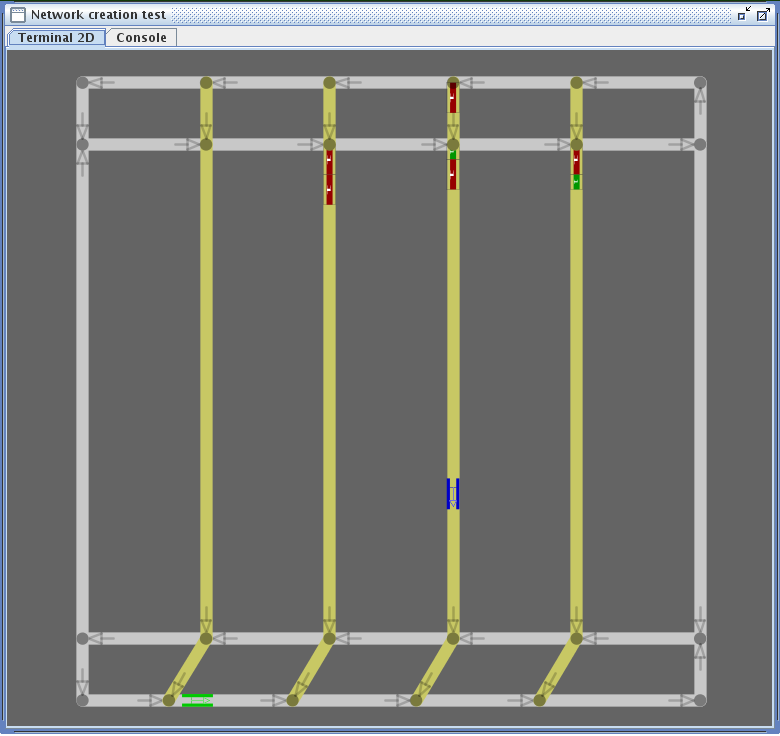
\includegraphics[height=3cm]{Shemas/terminal.png}
				\caption{Terminal view in the simulator}
				\label{tview}
			\end{center}
		\end{figurehere}
		\begin{figurehere}
		 	\begin{center}
				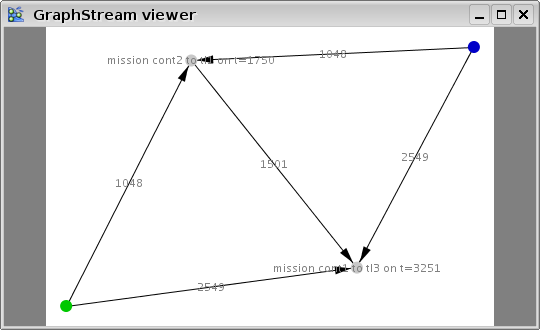
\includegraphics[height=2.5cm]{Shemas/acocapture.png}
				\caption{Mission graph view in the simulator}
				\label{acoview}
			\end{center}
		\end{figurehere}
		
		(The end of this part will be completed soon)
% 	\section*{Results}
% 	Coming soon !

	\section*{Conclusion}
	The problem to solve belongs to the Dynamic Pickup and Delivery Problem with Time Windows class. However, it does not exactly fit. So it is an original unsolved problem. We propose to solve it using swarm intelligence methods. An Ant Colony System is being developped. It uses colored ants and a graph modeling in order to plan a schedule.
	
	%\section*{Biliography}
	\bibliographystyle{plain}
	\bibliography{biblio}
\end{multicols}
\end{document}
